\section{Active light sources}
% According to Scott Palmer in his book Light (2013), passive and active light were at the core of Adolphe Appia's creative vision. 'The passive or diffused light refers to the general light of the stage area usually from footlights and border lights, which were common to existing stage practices at the end of the nineteenth century and were principally concerned with the widespread illumination of the stage space. In contrast, active light refers to intense, focused light that crucially allows distinct shadows to be created.
In 3D machine vision, there are many sources of light, used by the cameras to collect the information of interest. We can group these sources into two sets: \textit{passive} and \textit{active} sources. The first set refers to reflected light (typically used in photography), that is ``the general light of the stage area [\ldots] and were principally concerned with the widespread illumination of the stage space'' \cite{palmer2013light}. The second set refers to all intense and focused lights that create distinct shadows on the scene.
% Per quanto riguarda i sistemi basati su triangolazione ...
As far as triangulation-based systems are concerned, we are only interested in active sources, in particular in \acs{LASER}. \\

A \acs{LASER} is a device that emits a coherent light beam, and originally its name was the acronym of \textit{Light Amplification by Stimulated Emission of Radiation}. It comes from the physical processes used to generate the light beam: when an incoming photon (at a specific frequency) interacts with an excited electron, the electron changes its energy level. The energy liberated when it returns to its initial state, generates a new photon, completely identical to the first one. Now, the four main parts that compose this device are:
  \begin{itemize}
    \item The \textit{active medium} is the source of optical gain.
    \item The \textit{pumping system}, that provides the energy needed to excite photons.
    \item The \textit{cavity resonator}, where the photons are reflected back and forth between the cavity's walls.
    \item The \textit{collimator}.
  \end{itemize}
As far as the last point is concerned, it is not a fundamental element from the point of view of the \acs{LASER} itself, but for its use in measuring systems. In fact, as we will describe later, the emitted light has the shape of a spot. To spread it along a line, a collimator is needed. A collimator is a particular curved lens, putted in front of the \acs{LASER}, that filters the stream of rays so that only those travelling parallel to a specified direction are allowed through. In this way, it is possible to spread the light power on a plane and to obtain a \acs{LASER} line on the target.\\

The main properties of the \acs{LASER}s are their temporal and spatial coherences. The spatial coherence allows the \acs{LASER} to be collimated: this means that the rays of light are all parallel to each other, generating the typical shape of a spot. For this reason, in \acs{SOL} systems it is common to put a \textit{collimator} in front of the \acs{LASER}, in this way the energy of the collimated spot is spread to a plane, that is a line when it hits a target object. \\
Temporal coherence, instead, allows the \acs{LASER} to emit light with a very narrow spectrum, i.e. they are monochromatic. \\
Thanks to their coherencies, the \acs{LASER}s can focus a great amount of energy on a very small areas, allowing their use in a wide range of applications. Depending on the field of application, we can find \acs{LASER}s with different wavelengths, both in visible and invisible spectrum. \\

  \begin{table}[b!]
  \begin{tabular}{|c|p{12cm}|}
  \hline
  \multicolumn{1}{|c|}{\textbf{Class}} & \multicolumn{1}{c|}{\textbf{Description}} \\
  \hline
  
  1  &
  \acs{LASER}s that belong to this class are always safe for the human health. Generally the emitted power is $P < 0.04 mW$, but in this class there are also that \acs{LASER}s that prevents the direct interaction of the operator (such as laser printers). No protection is required. \\
  \hline
  
  1M &
  This class differs from the previous one because these are dangerous \acs{LASER}s, if used in pair with optical instruments. Typically, their works in the range $\left[302.5, 4000\right] nm$. \\
  \hline
  
  2  &
  These are low-power \acs{LASER}s $\left( P < 1 mW\right)$ that emit in the visible spectrum $\left( 400, 700 \right) nm$. This type of \acs{LASER}s are not inherently safe, but the eyelid is enough to protect eyes from incidental reflections. It is important not to look them directly. \\
  \hline
  
  2M &
  Like the class 1M, \acs{LASER}s belonging to this class refer to class 2 too, but are dangerous if used in pair with optical instruments. \\
  \hline
  
  3R &
  This is the first class of \acs{LASER}s that are really dangerous for humans. Here we find \acs{LASER}s that emit in the visible spectrum $\left(302.5, 106\right) nm$. They can injure eyes even if viewed indirectly. \\
  \hline
  
  3B &
  Like the class 3R, we can find \acs{LASER}s dangerous both for eyes and skin. They emit beams with power under $500 mW$. \\
  \hline
  
  4  &
  Like the class 3B, \acs{LASER}s that belong to this class are dangerous for eyes and skin, even in diffuse radiation, and they can cause fires. Another source of danger are their very high working voltage and current. We have to be very careful when we use this class. \\
  \hline
  \end{tabular}
    
  \caption{Classes of \acs{LASER}s and their regulations} 
  \label{tab:laser-classes}
\end{table}
Nevertheless, lasers coherence can be a risk factor for the health of users. Because of their differences in wavelength, emitted power and pulse frequencies, it has been necessary to rule their use, and to group them, accordingly with their properties. \acs{CEI} grouped \acs{LASER}s in five classes, accordingly with regulations \cite{cei:76-2}, in order to define the \acs{MPE} (Maximum Permissible Exposure) for each category, i.e. the maximum exposure time in which the damage for the health is negligible. These classes are described in Table \ref{tab:laser-classes}. The choice of the correct class needed in our project is very important, in particular in industrial systems. For our tests, described later, we used \acs{LASER}s belonging to classes 1 and 2. \\

% --------------------------- %
\subsection{Peak detection}
\label{subsec:peak-detection}
An important aspect of lasers is their mathematical modelling. The accuracy of triangulation-based systems, and in general of laser-based systems, is significantly determined by the detection of the laser stripe. \\

In literature there are many models that try to describe laser stripes, but the most used is the \textit{Gaussian} shape that, accordingly with \cite{saleh2013fundamentals}, we can generalize as:
  \begin{equation}
    e^{-jkz}
    \label{eq:general-gauss-model}
  \end{equation}
where $k = \frac{2\pi}{\lambda}$ is the wavenumber with wavelength $\lambda$, and $z$ is the direction of propagation of the signal. This model is quite simple, because it approximates the spot laser with the point of maximum light intensity (peak of the Gaussian). Furthermore this model is symmetrical with respect to the center of the spot, guaranteeing the shape shown in Figure \ref{fig:laser-spot-gauss}. Like camera lenses, also lasers have to be focused. Since the beam has its minimum width at $z = 0$, this will be the best focus plane. Moving in both directions, the width of the beam grows ``out of focus''. When the width of the beam is $\sqrt{2}$ the initial width, we have reached the laser \textit{depth of focus}.
  \begin{figure}[t!]
  \centering
    \begin{minipage}[c]{.48\textwidth}
      \centering
      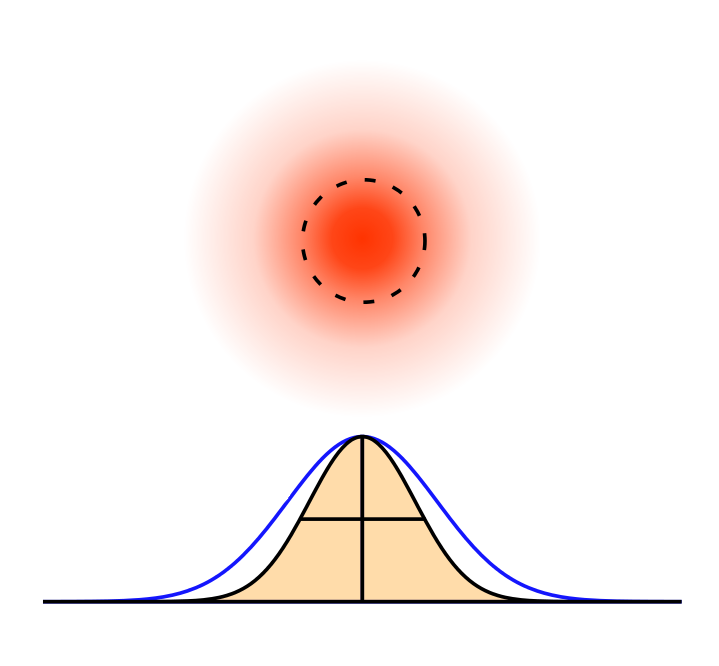
\includegraphics[width=0.8\textwidth]{./images/tech/laser-gauss.png}
      \subcaption{Gaussian model.}
      \label{fig:laser-spot-gauss}
    \end{minipage}
    \hfill
    \begin{minipage}[c]{.48\textwidth}
      \centering
      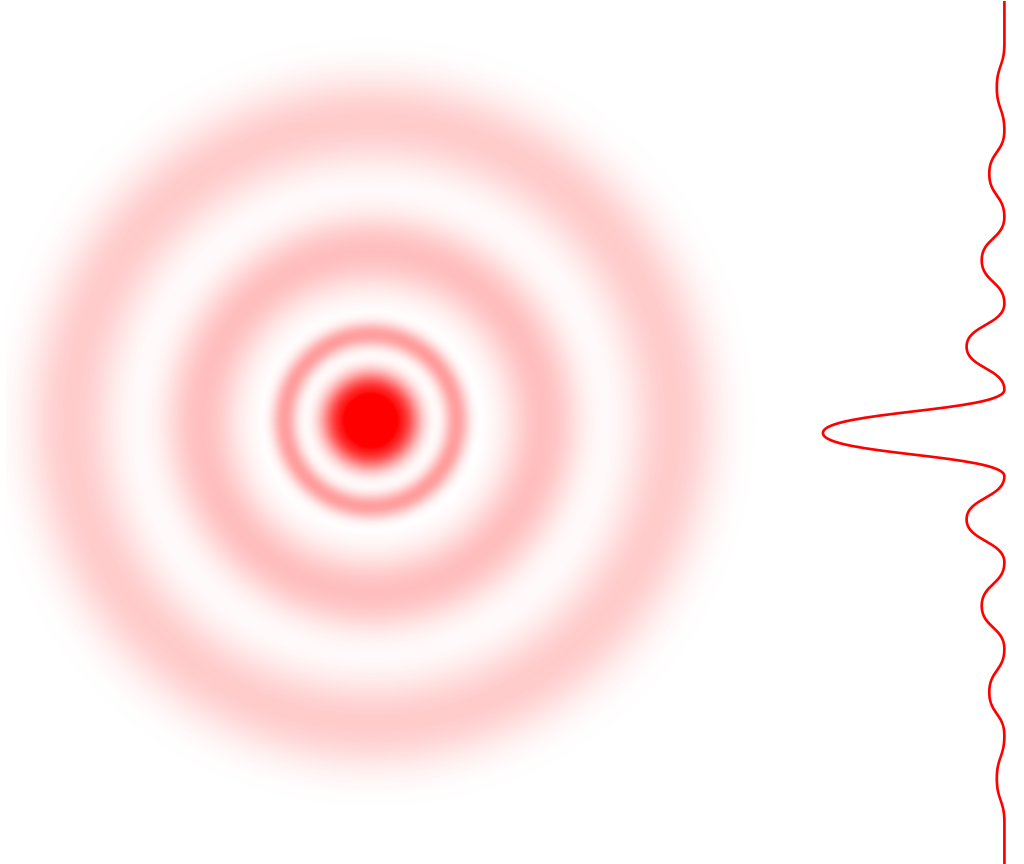
\includegraphics[angle=270, origin=c, width=0.64\textwidth]{./images/tech/laser-bessel.png}
      \subcaption{Bessel model.}
      \label{fig:laser-spot-bessel}
    \end{minipage}
    \caption{Models for lasers spots.}
    \label{fig:laser-spot-models}
  \end{figure}

Another solution, proposed in \cite{saleh2013fundamentals}, is the \textit{Bessel} laser model. As we can see in Figure \ref{fig:laser-spot-bessel}, this model is very similar to the Gaussian one: it has a global maximum and it is symmetrical with respect to its center. The interesting thing is the fact that it is diffraction free and has a bigger depth of field than the Gaussian model. \\

Before going deeper in the problem of laser extraction from an image, it is important to introduce the \textit{speckle noise}. Speckle noise is a granular noise that inherently exists in all coherent sources (lasers, radars, SAR, ...). It is generated when a coherent signal strikes a rough surface, spreading random radiation into space. Thanks to their coherence, the radiations are identical to the original signal, but some of them change their phase, interfering with each other. The interferences can be constructive or destructive, and what we see in the image plane is a dotted spot. The effects of this noise change if we vary the wavelength of the laser, the aperture of the lens and the setup of triangulation system, but the main important thing is that, accordingly with \cite{Baribeau:91},\cite{Dorsch:94} and \cite{Hausler:88}, this noise is a limit for the determination of the precise position of the spot in the image. \\

Once we have defined these models, the next step is to locate the laser position in the image. To do that, we can consider each row of the image as a Gaussian, defined by the value of the pixel belonging to that row, as shown in Figure \ref{fig:tech:laser-prof}. Thanks to shape and symmetry of the Gaussian distribution, it is common to look for the pixel of greatest light intensity, that ideally is located under the peak of the laser. Using this approach for each row of the same frame, we can obtain the results shown in Figure \ref{fig:tech:laser-example}.
%Once we have defined these models, the next step is to locate the laser position in the image. To do that, we can consider each row of the image as a Gaussian, defined by the value of the pixel belonging to that row. In Figure \ref{fig:tech:laser-prof} we shown a representation of this assumption. Thanks to shape and symmetry of the Gaussian distribution, it is common to look for the pixel of greatest light intensity, that ideally is located under the peak.
% Once we have defined these models, the next step is to locate the laser position in the image. Thanks to their shape and symmetry, it is common to look for the pixel of greatest light intensity, that ideally is located under the peak.
However, as we can see in Figure \ref{fig:gauss-discr} this is not completely correct: the discretization introduced by the physical structure of the sensor, forces the Gaussian to stay in the middle of the pixel, and in some cases (such as the one illustrated in Figure) if the peak is between two pixels, we make an error regardless of the pixel we choose. From the point of view of the accuracy of the measure, this approximations are too coarse to satisfy the typical industrial requirements. \\

  \begin{figure}[t!]
    \centering
    \begin{minipage}{\textwidth}
      \centering
      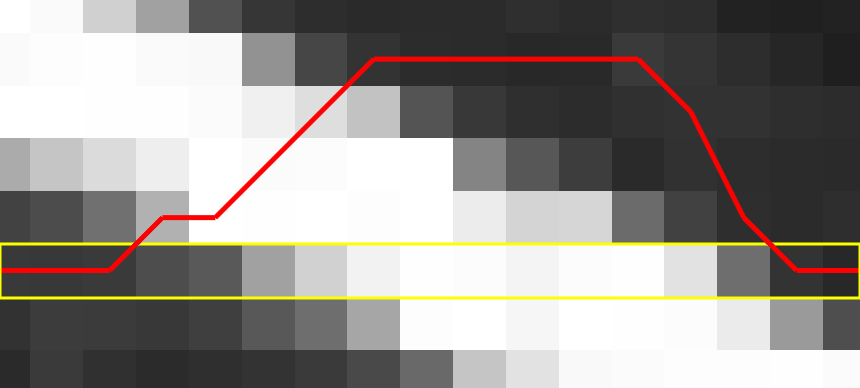
\includegraphics[width=0.8\textwidth]{./images/tech/laser_prof.png}
      \caption{Gaussian approximated distribution of the highlighted line.}
      \label{fig:tech:laser-prof}
    \end{minipage}
    \vfill
    \begin{minipage}{0.49\textwidth}
      \centering
      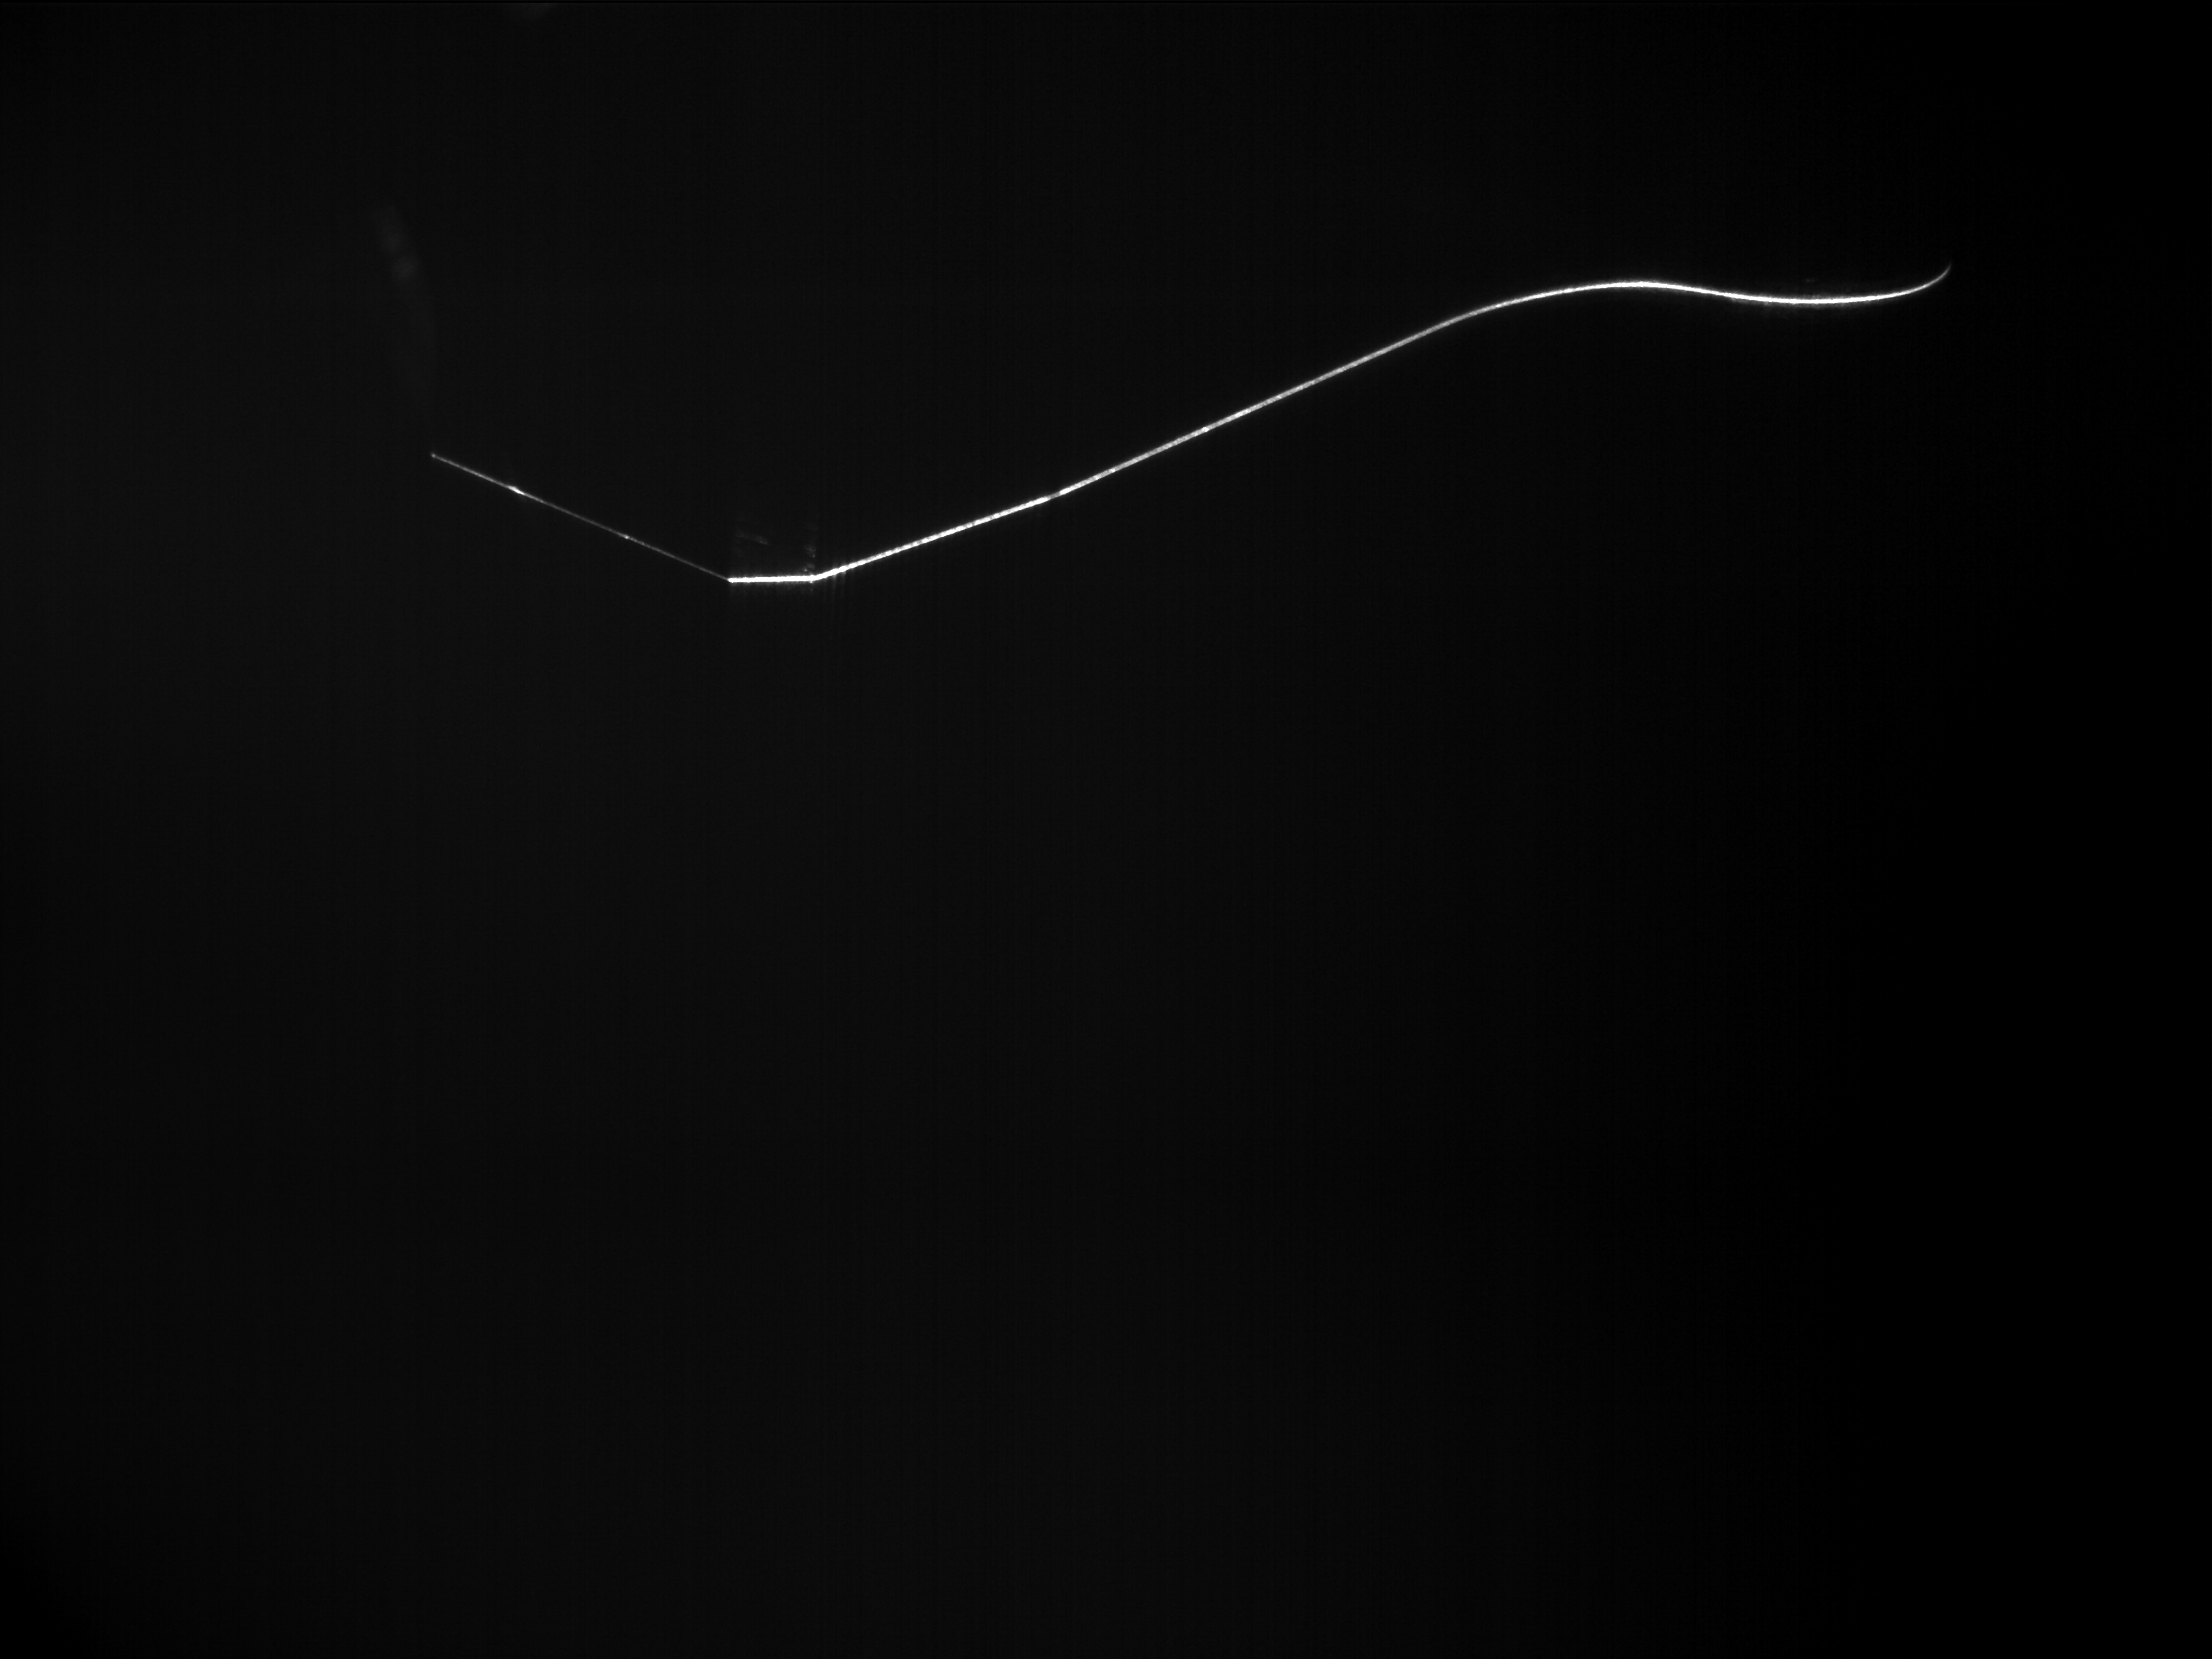
\includegraphics[width=\textwidth]{./images/tech/C0_p240_SD.png}
    \end{minipage}
    \hfill
    \begin{minipage}{0.49\textwidth}
      \centering
      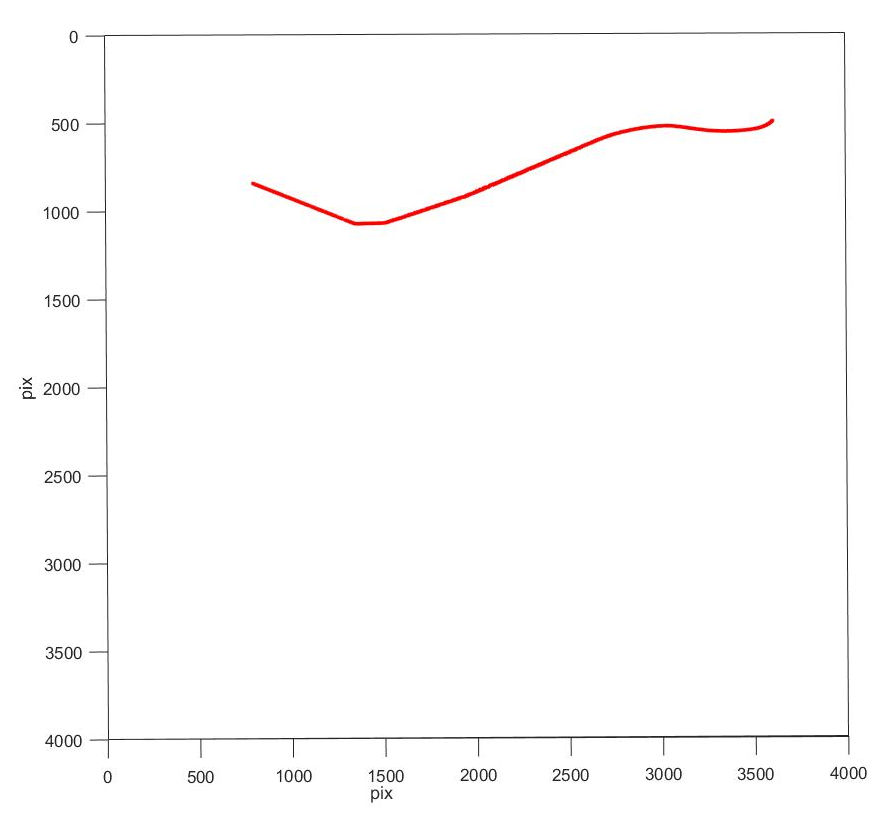
\includegraphics[width=0.9\textwidth]{./images/tech/profile_ex.jpg}
    \end{minipage}
    \caption{Example of profile extraction. On the left there is a live frame of a railway wheel, while, on the right, there is the extracted profile.}
    \label{fig:tech:laser-example}
  \end{figure}
\vfill
  \begin{figure}[t!]
    \centering
    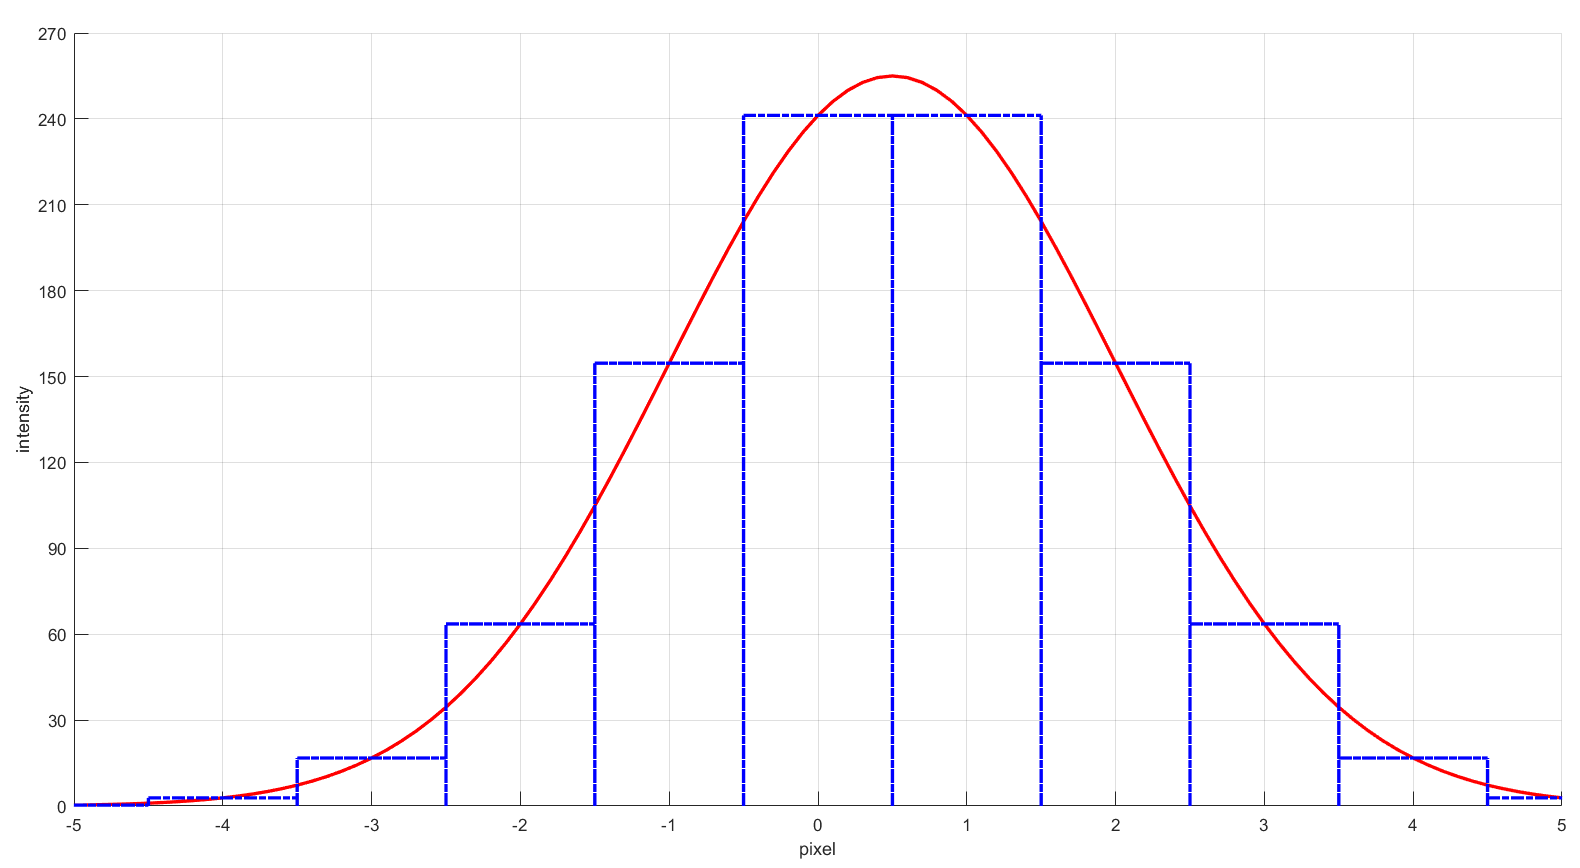
\includegraphics[width=0.79\textwidth]{./images/tech/gauss-discr.png}
    \caption{Gaussian distribution discretization because of pixels.}
    \label{fig:gauss-discr}
  \end{figure}

To try to solve these problems, in literature we can find a lot of solutions, such as in \cite{BLAIS1986145}\cite{Dorsch:94}\cite{1334612}\cite{Naidu1991}\cite{doi:10.1080/095119298130642}.
All of the proposed filters try to approximate the shape of the Gaussian model, starting from the light intensities collected by the pixels, and in this way the peak location with subpixel accuracy is improved. \\
To better understand how these filters works, we grouped them in two categories:
  \begin{itemize}
    \item the first one gathers all that filters that use mathematical relations to fit a Gaussian distribution over the pixels;
    \item the second one gathers all that filters that compute the discrete derivatives of the discrete signal, and use them to locate the global maxima.
  \end{itemize}
Given the pixel collected by the greatest amount of light intensity, all the filters described below locate the peak of the spot using only the pixels along the $y$ axis, consistently with the coordinate reference system used in Section \ref{sec:init-modelanalysis} (parallel to the direction of the laser beam).

In the following of this section, we will indicate with $y$ the coordinates of the pixel candidate to contain the peak of the spot laser, while with $b$ the light intensity collected by that pixel. Then we will indicate with $a$ and $c$ the light intensities collected by the pixels $y-1$ and $y+1$, respectively.

% --------- %
\subsubsection{Centre of Mass (\acs{COM})}
The \acs{COM} (known as \textit{Center of Gravity}, \acs{COG}) is probably the most used subpixel filter. It tries to determine the peak of a gaussian distribution implementing a sliding window mean. Given $a$, $b$ and $c$, we can write:
  \begin{equation}
    \hat{Y} = y +\frac{c - a}{a + b + c}
    \label{eq:sp-com}
  \end{equation}
In literature, it is known that this filter is very sensitive to the noise in the image, in particular it is sensitive to the thermal noise.

% --------- %
\subsubsection{Gaussian approximation}
This filter is based on the idea that the laser spot is similar enough to a Gaussian distribution: as we will see later, this condition is never satisfied because of the thermal noise of the camera. Mathematically, the peak is given by:
  \begin{equation}
    \hat{Y} = y - \frac{1}{2}\left( \frac{\ln{c} - \ln{a}}{\ln{a} - 2\ln{b} + \ln{c}} \right)
    \label{eq:sp-gauss}
  \end{equation}
As we can see, this filter uses only three pixel to determine the position of the peak.

% --------- %
\subsubsection{Linear Interpolation}
Linear interpolation filter simply assumes that a linear relation exists among the usual three points
  \begin{equation}
    \hat{Y} = \begin{cases}
      y - \frac{a - c}{2(b - a)} \qquad if \quad c > a \\
      y - \frac{a - c}{2(b - c)} \qquad otherwise \\
    \end{cases}
    \label{eq:sp-linear}
  \end{equation}

% --------- %
\subsubsection{Parabolic Estimator}
Unlike the previous filter, the parabolic estimator tries to use a continuous vision of the laser signal, so it derives from the Taylor decomposition of the light intensity near the peak.
Let $\delta \in \left[ -\frac{1}{2}, \frac{1}{2} \right]$ be the variation of the peak position with respect to the center of the pixel $y$, and let $f(y + \delta)$ the real value of the peak. Thus, we can write:
  \begin{equation}
  \delta = \frac{f'(y)}{f''(y)} = \frac{f(y+1) - f(y-1)}{2\left( f(y+1) - 2f(y) + f(y+1)\right)}
    \label{eq:sp-parabolic}
  \end{equation}

% --------- %
\subsubsection{Blais and Rioux Detectors}
This filter was originally proposed in \cite{BLAIS1986145}. The original idea was to use a linear interpolator in cascade on a finite impulse asymmetrical digital filter. The authors obtained a linear filter insensitive to laser spot amplitude and, at least theoretically, more robust with respect to the \acs{COM}. Let $f(y)$ be the same function defined for the parabolic estimator, and let $g_d(i)$ a function defined as:
  \begin{equation*}
    g_d(i) = \sum_{k=-d/2}^{-1} f(i + k) - \sum_{k=1}^{d/2} f(i + k)
  \end{equation*}
The estimation of the peak position is given by
  \begin{equation}
      \delta = \frac{g(y)}{g(y) - g(y+1)} 
    \label{eq:sp-br}
  \end{equation}
if $f(y+1) > f(y-1)$; otherwise we will write: $\delta = \frac{g(y-1)}{g(y-1) - g(y)}$.
  
% --------- %
\subsubsection{FIR filter approach}
The last filter we are interested in, is the FIR. As a FIR filter, this one tries to evaluate the discrete derivative of the Gaussian distribution, and looks for the point in which the derivative intersects the origin: that point will be the peak position. We can use the following relation to describe what said so far:
  \begin{equation}
    \hat{Y} = y_0 - \frac{I_0 \cdot \left( y_1 - y_ 0\right)}{I_1 - I_ 0}
    \label{eq:sp-fir}
  \end{equation}
where $I_i$ is the intensity of light collected by the sensor in the pixel; $(y_0, I_0)$ are the coordinate and the intensity of the last point before the origin, while $(y_1, I_1)$ are the coordinate and the intensity of the first point after the origin.

Also in this case, we assume that the error committed locating the peak position is at most half pixel. \\

\bigskip
As we can see, all the filters above are introduced using only three pixels. In real systems this could not be enough to reach a good precision in the measures, generally because of the depths of field of cameras and lasers. Moreover, laser beams can be as thick as $30$ pixels: in these cases, considering only three pixels makes the final approximation very partial, and in saturation conditions the problem is what pixels must be considered. Furthermore, as just mentioned, they are sensitive to the presence of noise in the image. In particular, the thermal noise (described in Subsection \ref{subsec:overview-cameras}) has to be removed before to exploit subpixels optimizations, for example subtracting the background noise of the camera.
Accordingly with \cite{1334612} and \cite{Naidu1991}, Filters \ref{eq:sp-gauss}, \ref{eq:sp-linear}, \ref{eq:sp-parabolic}, \ref{eq:sp-br} and \ref{eq:sp-fir} should be better than \ref{eq:sp-com}, but our analysis shown something different.
